\newpage
\section{RESULTS}

\hspace{5mm} After the final program was coded, the result obtained was close to what was expected. Game uses keyboard keys for function. Program starts with a short Intropage (for 2 sec) and then Mainmenu loads-up, with Play, HighScore, and Exit buttons. When played, the game goes into play state and game runs.\\ 

When the user gets out, GameOverState loads-up, and he is asked his name for storing his scores in a File. Then he can view top-ten scores in by pressing HighScore button and can press backspace to return back to the mainmenu state.\\
Then  pressing the Exit button will close the gameplay window.\\

\begin{figure}[H]
	\centering
	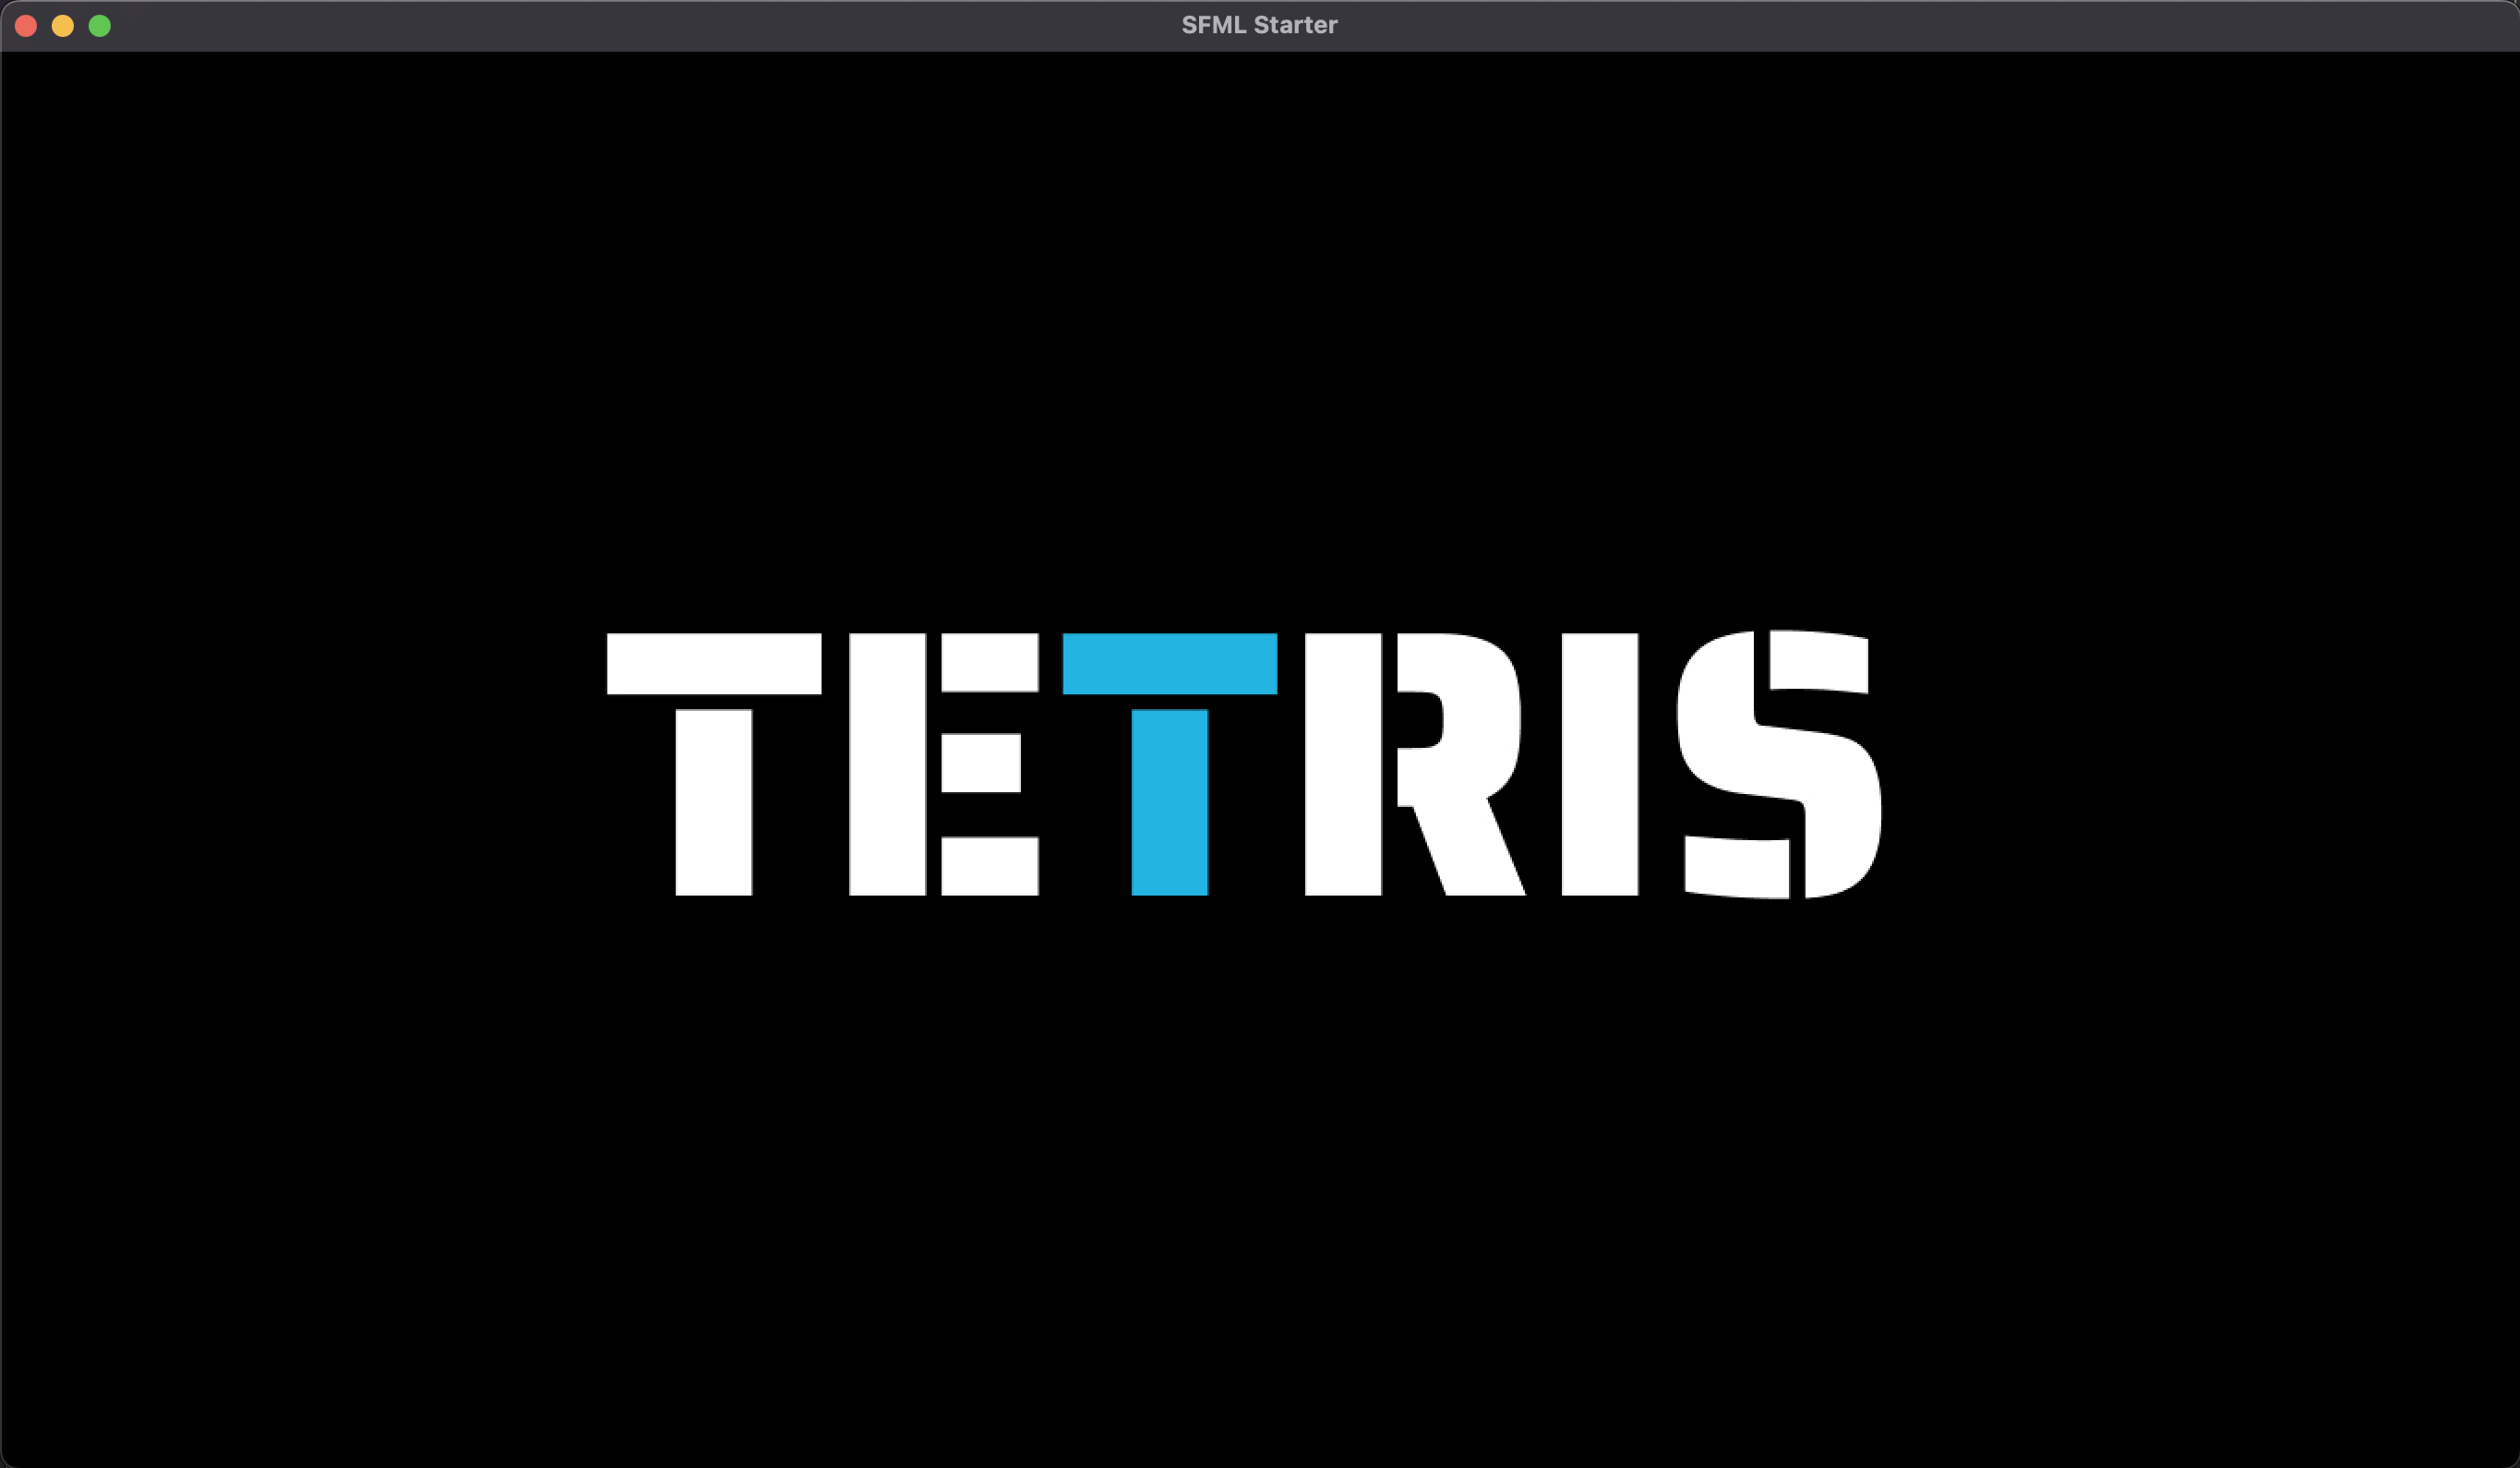
\includegraphics[width=0.9\textwidth]{images/IntroState}
	\caption{IntroState}
\end{figure}

\begin{figure}[H]
	\centering
	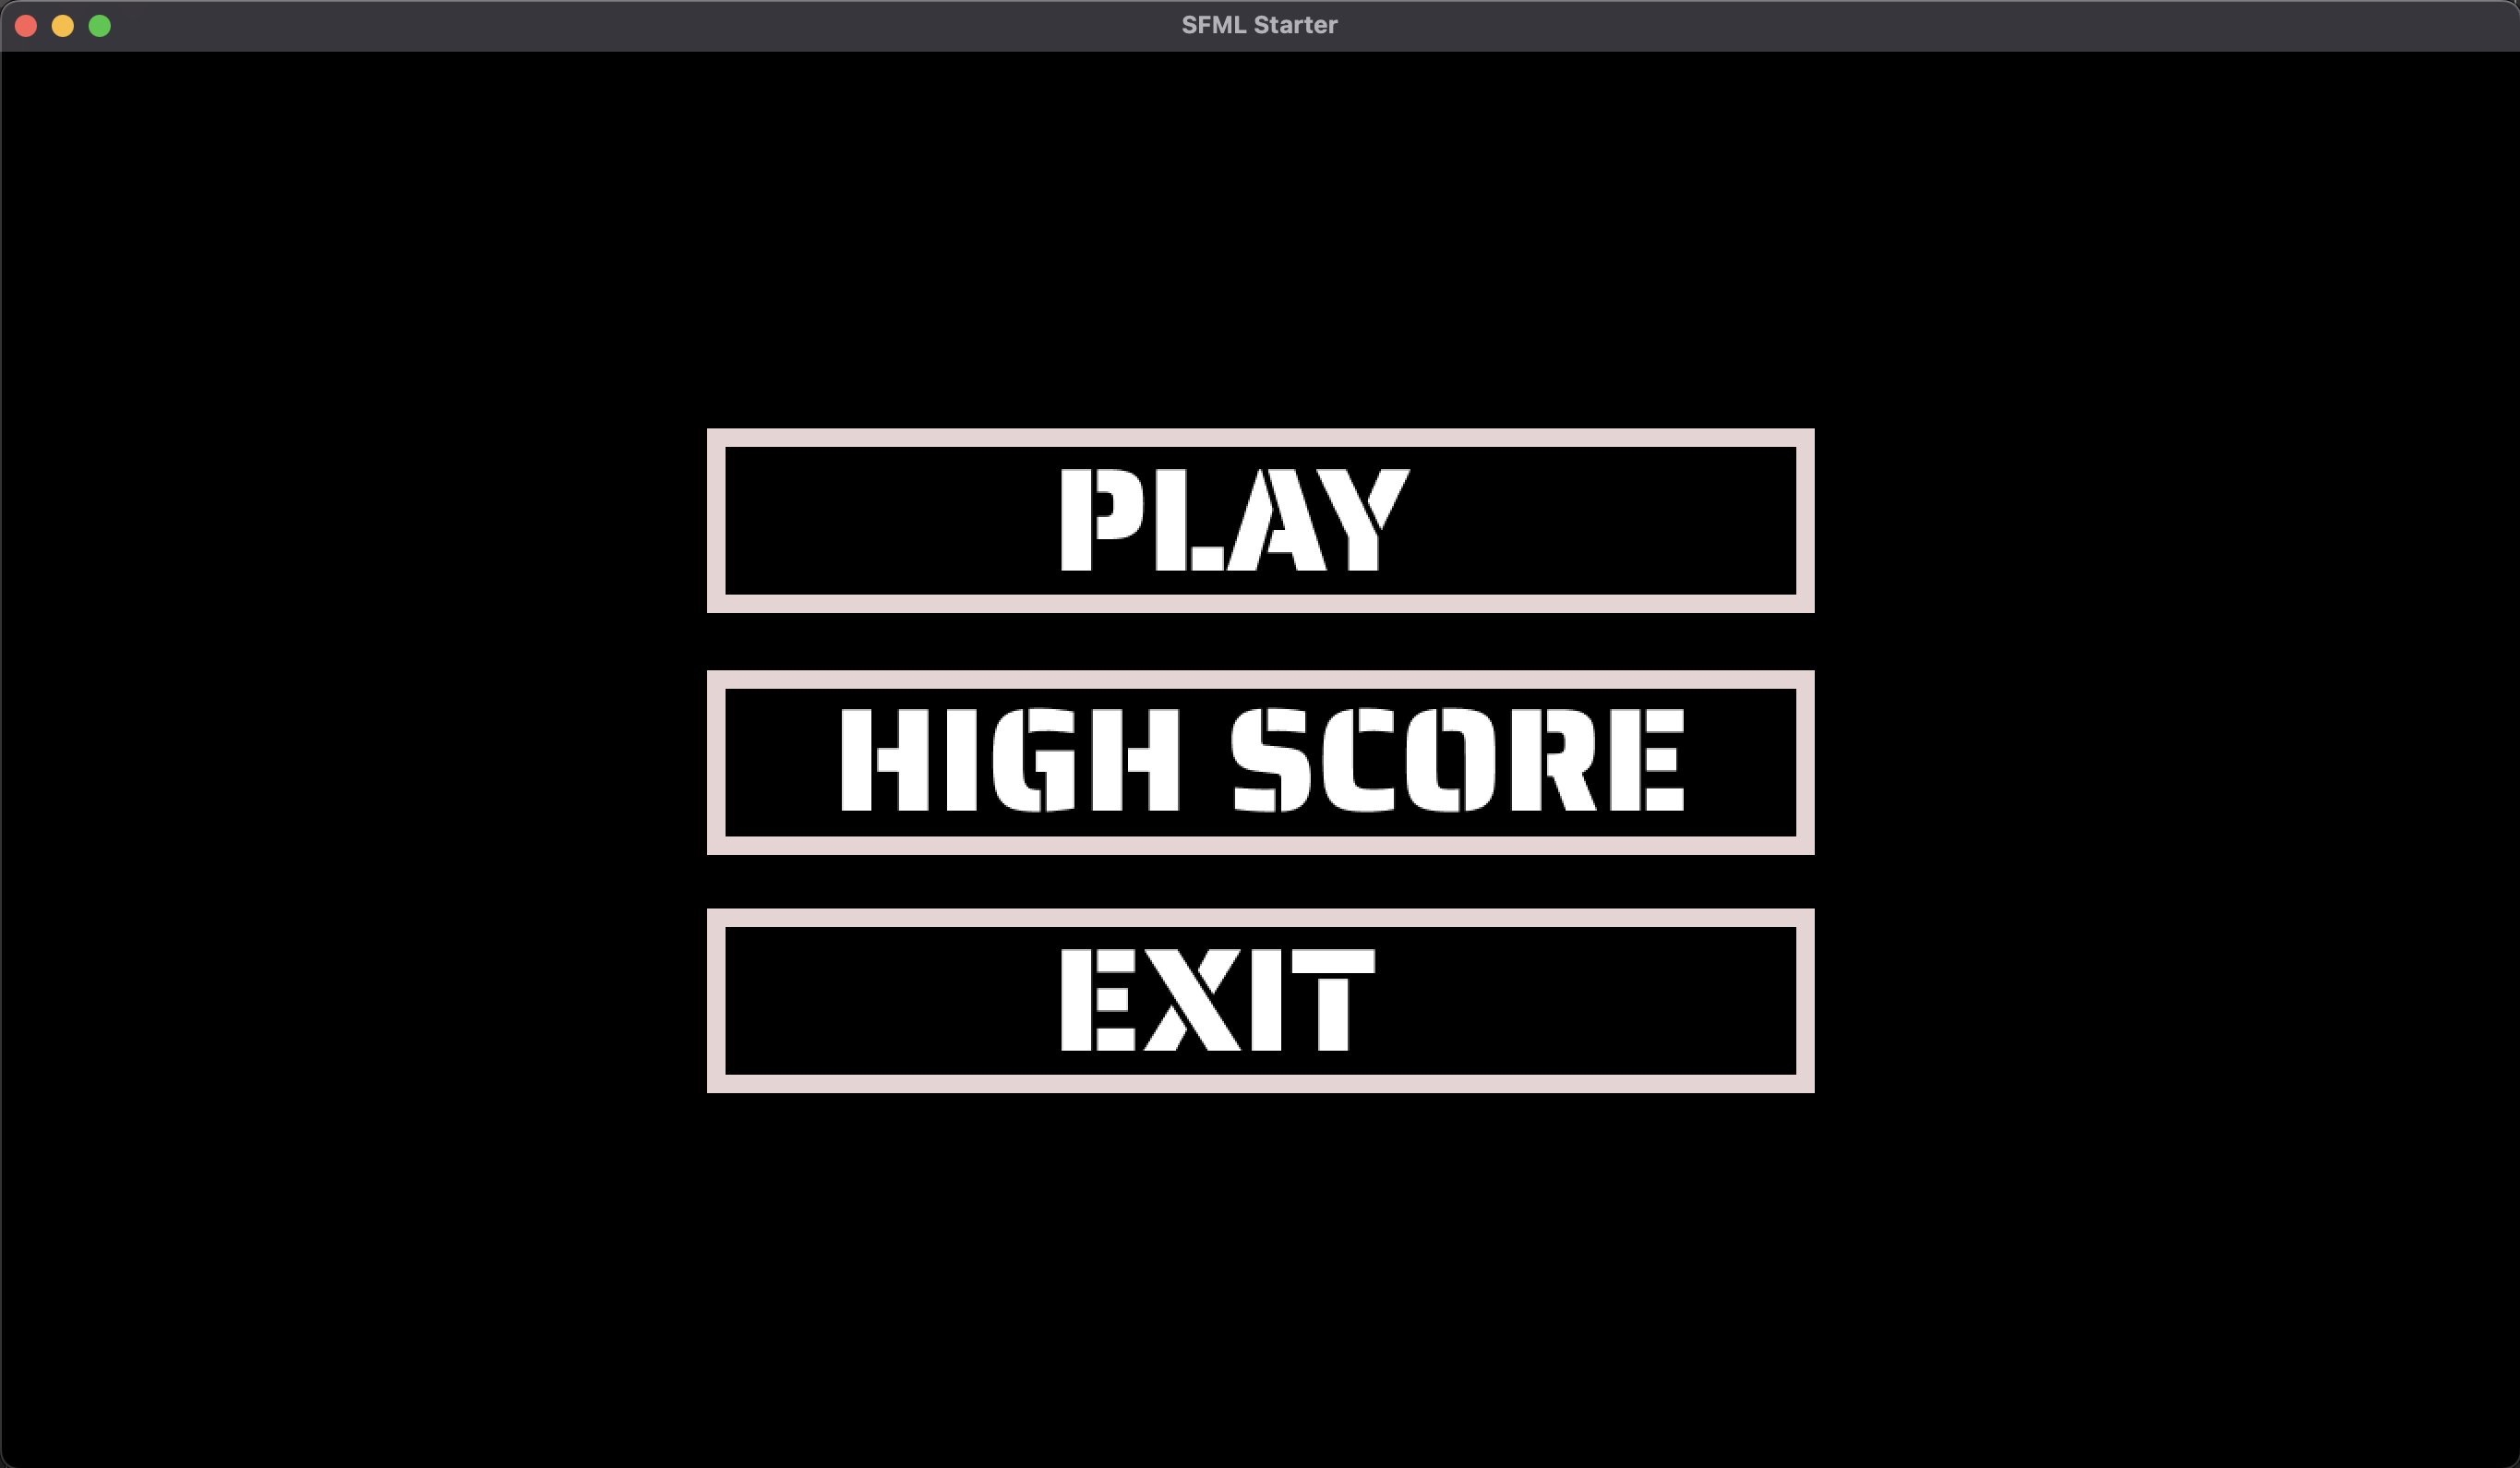
\includegraphics[width=0.9\textwidth]{images/MainMenuState.png}
	\caption{MainMenuState}
\end{figure}

\begin{figure}[H]
	\centering
	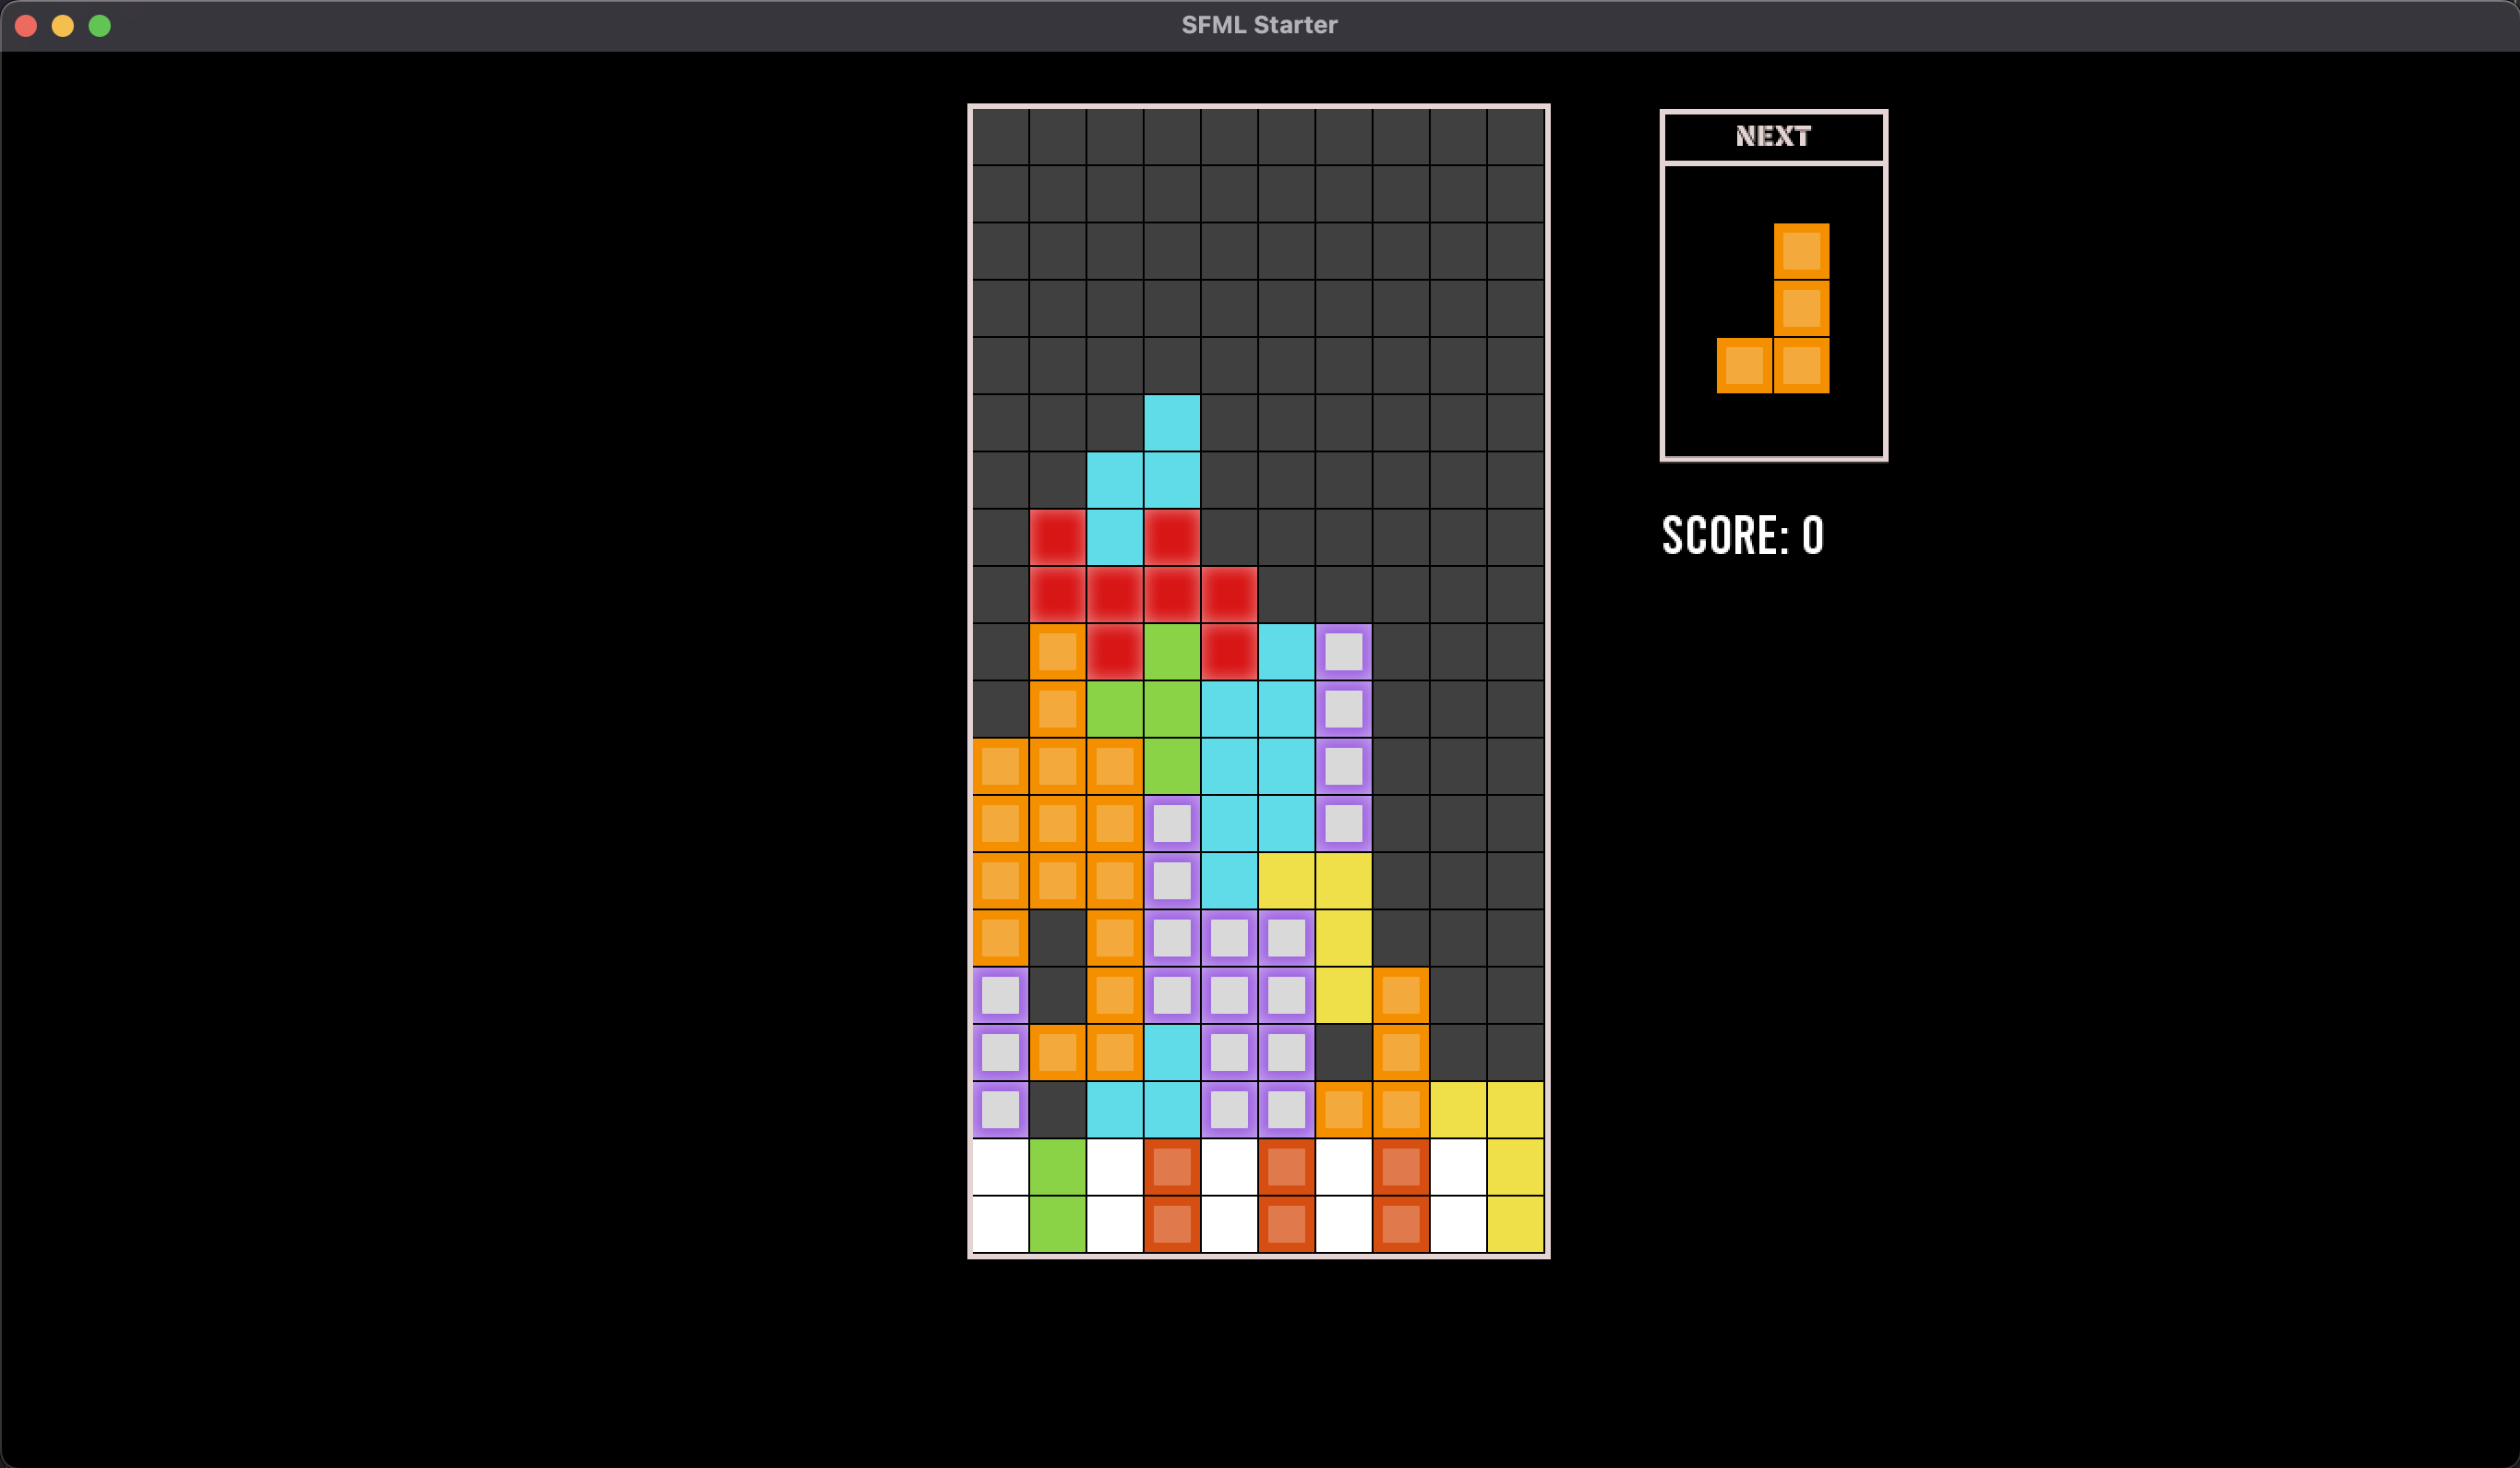
\includegraphics[width=0.8\textwidth]{images/GamePlayState.png}
	\caption{GamePlayState}
\end{figure}
\begin{figure}[H]
	\centering
	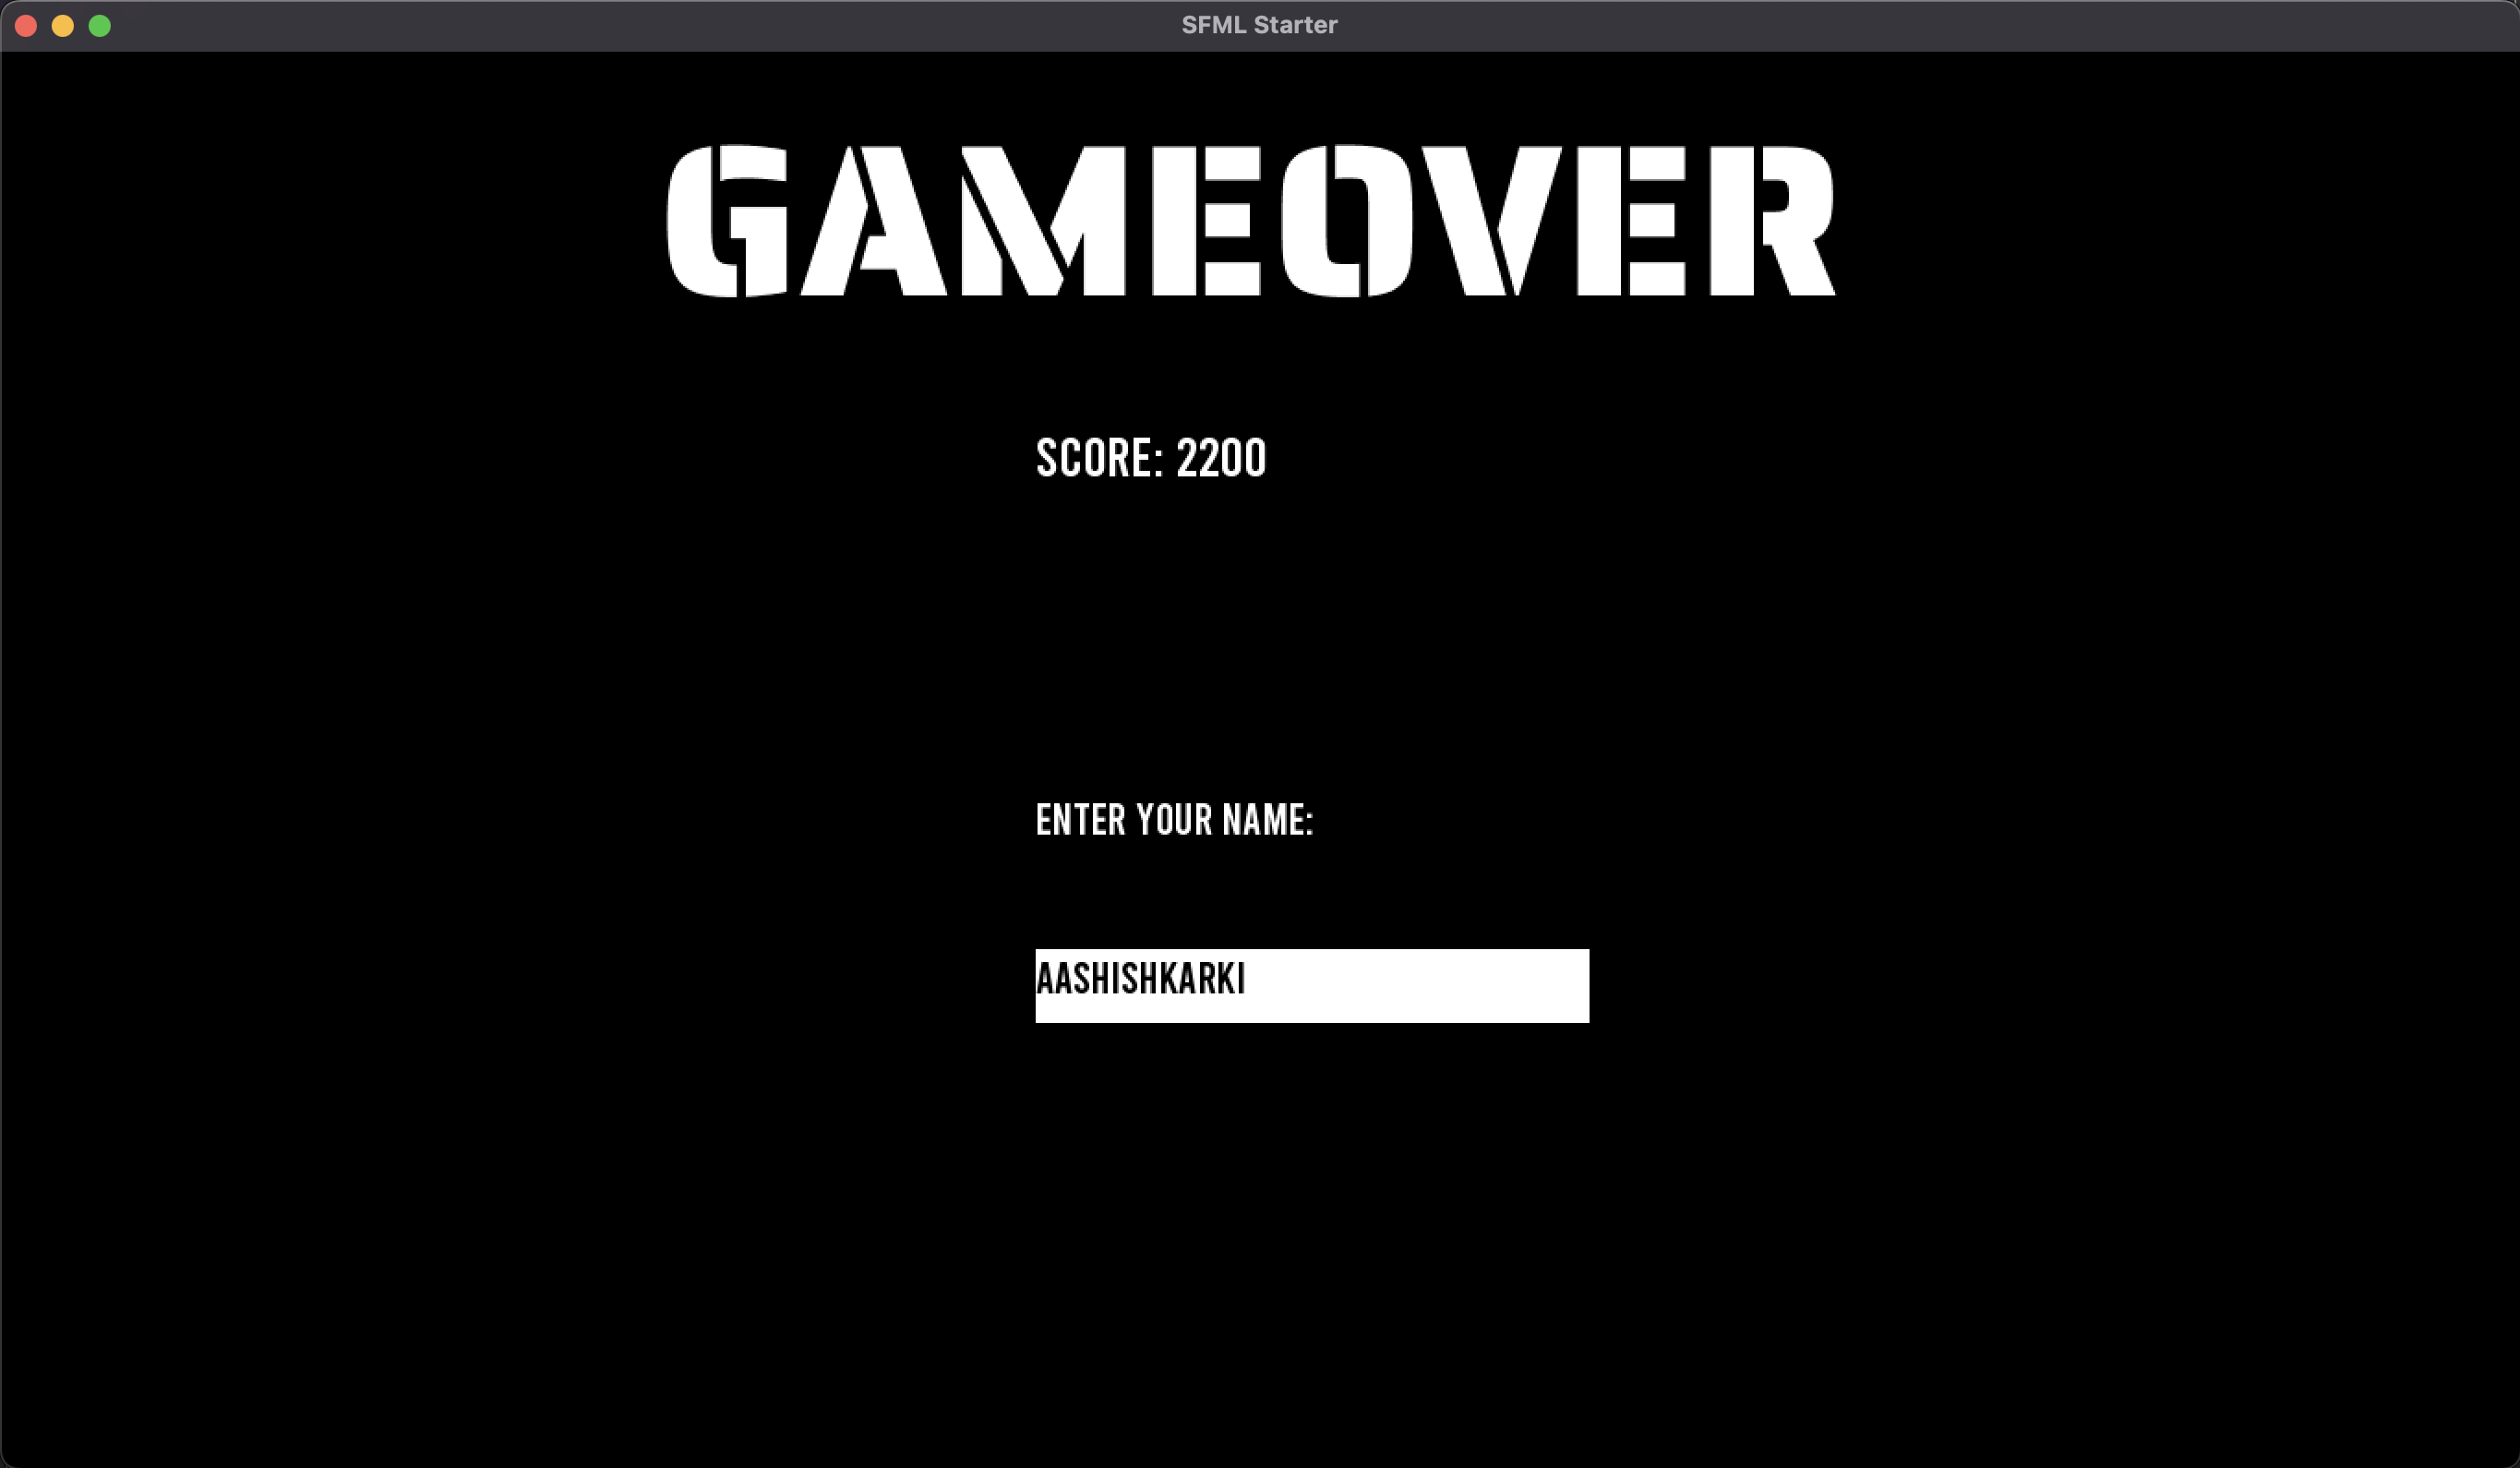
\includegraphics[width=0.8\textwidth]{images/GameOverState.png}
	\caption{GameOverState}
\end{figure}
\begin{figure}[H]
	\centering
	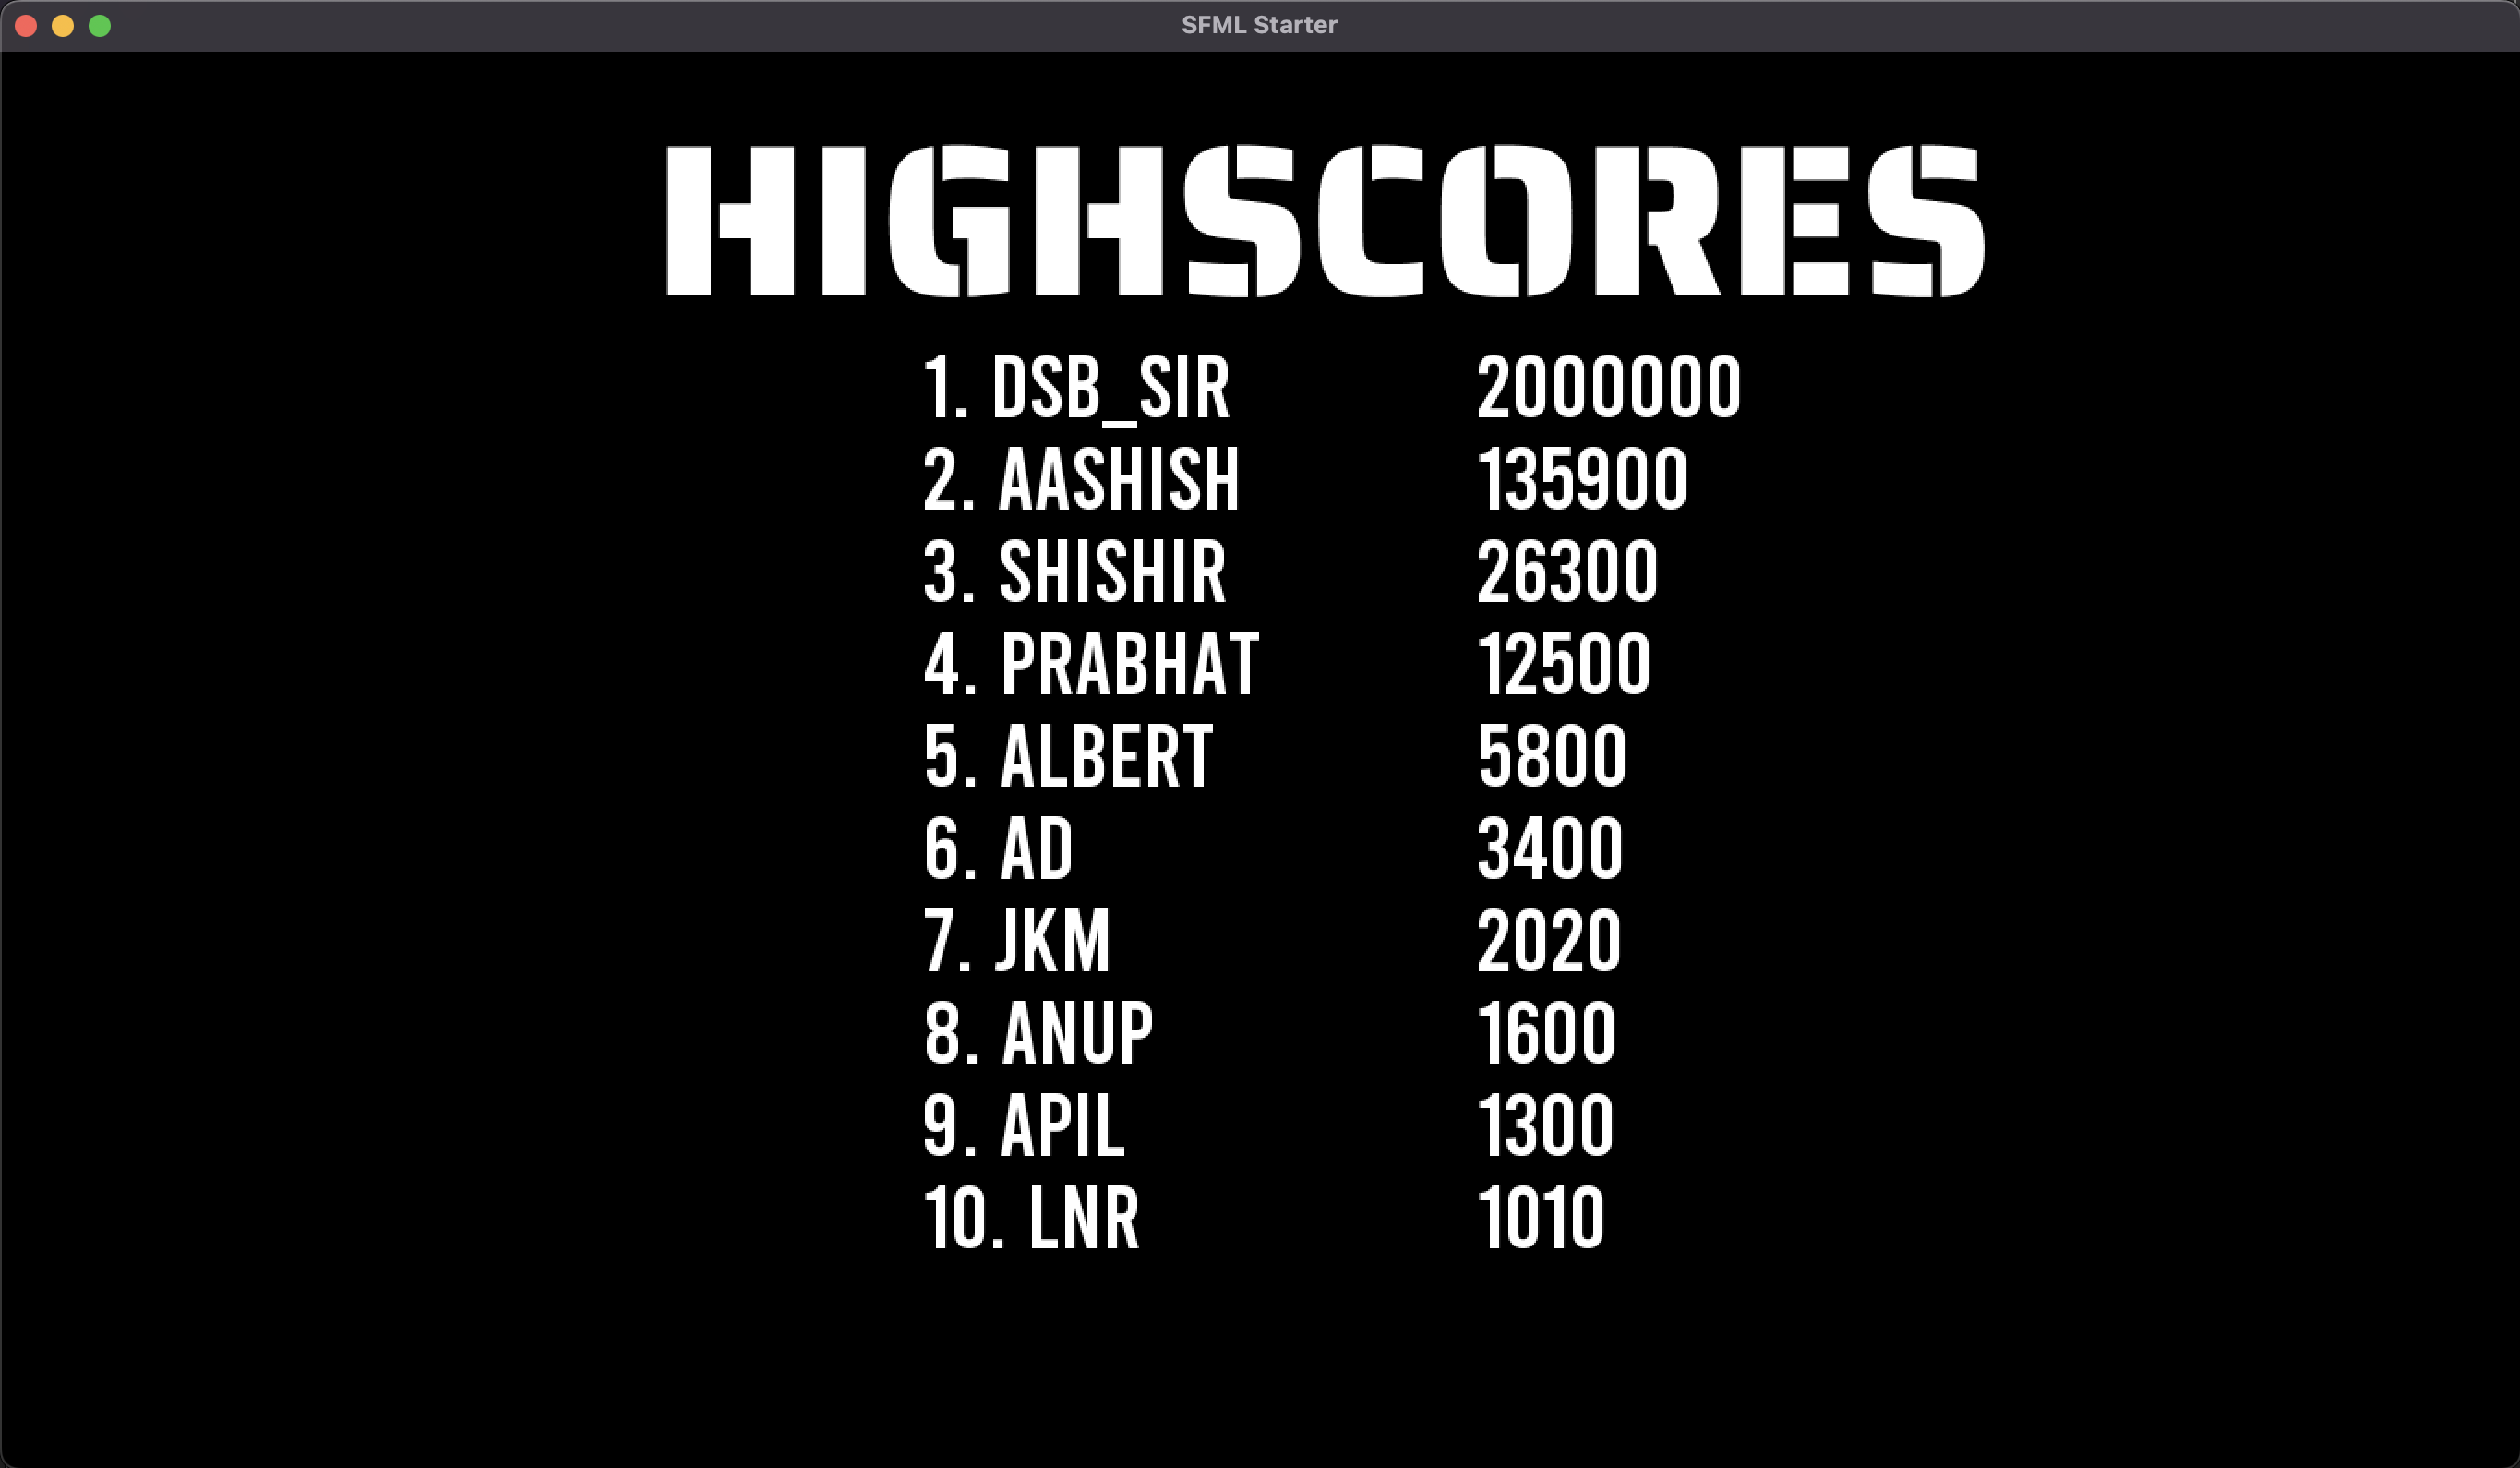
\includegraphics[width=0.8\textwidth]{images/HighScoreState.png}
	\caption{S}
\end{figure}

